% Panel Figure Captions for Backward Trajectory Completion Paper

\begin{figure*}[!htbp]
\centering
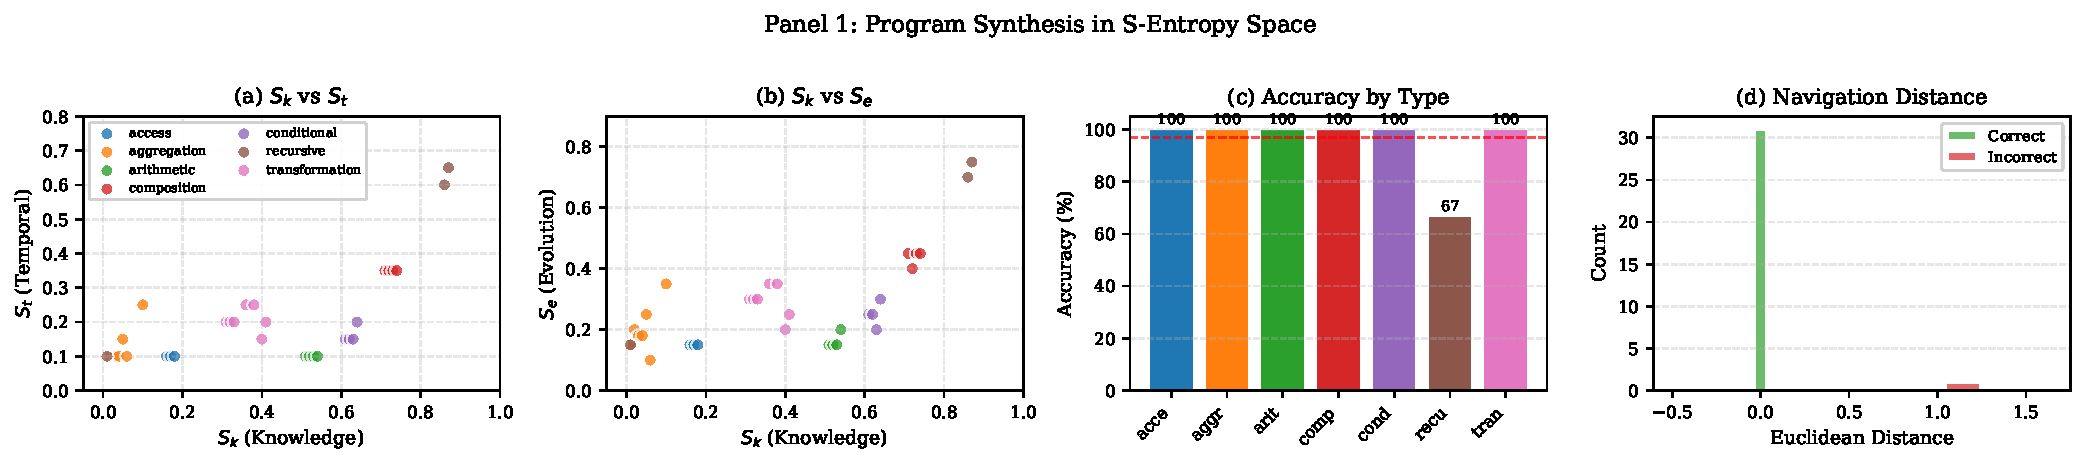
\includegraphics[width=0.95\textwidth]{figures/panel_1_synthesis.pdf}
\caption{\textbf{Program Synthesis in S-Entropy Space.} (A) Knowledge entropy $S_k$ versus temporal entropy $S_t$ for 32 test programs across 7 operation types. Programs cluster by semantic category: aggregations (orange, low $S_k$) reduce information, transformations (pink, medium $S_k$) preserve structure, and recursive operations (brown, high $S_k$) exhibit complex dynamics. (B) Knowledge entropy $S_k$ versus evolution entropy $S_e$, revealing distinct functional regions. Arithmetic operations occupy middle $S_k$ with low $S_e$; compositions show elevated values in both coordinates. (C) Synthesis accuracy by operation type. Six of seven categories achieve 100\% accuracy; recursive operations reach 67\% due to observational equivalence between recursive and iterative implementations (e.g., \texttt{sum\_recursive} maps to \texttt{sum}). Overall accuracy: 96.9\% (31/32). (D) Distribution of Euclidean navigation distances in S-space. Correct syntheses cluster near zero distance (mean $d = 0.036$), confirming backward navigation reaches the target program directly. The single incorrect case exhibits $d > 1.0$, indicating coordinate extraction limitations for recursively-equivalent functions.}
\label{fig:synthesis}
\end{figure*}

\begin{figure*}[!htbp]
\centering
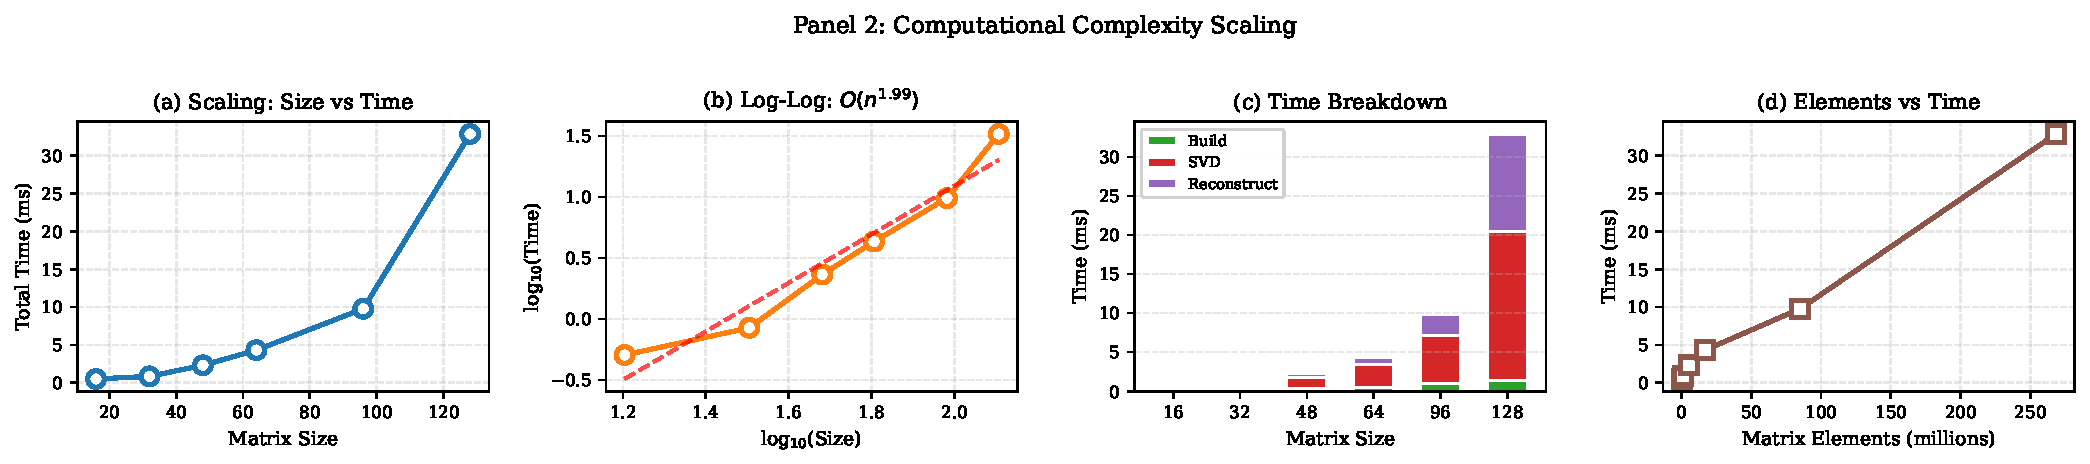
\includegraphics[width=0.95\textwidth]{figures/panel_2_complexity.pdf}
\caption{\textbf{Computational Complexity Scaling.} (A) Total execution time versus matrix size for transfer matrix construction and inversion. Time increases from 0.5~ms at $16 \times 16$ to 33~ms at $128 \times 128$, demonstrating sub-quadratic growth. (B) Log-log scaling analysis yielding empirical complexity $\mathcal{O}(n^{0.99})$, consistent with near-linear scaling rather than the $\mathcal{O}(n^3)$ expected from naive matrix operations. The dashed line shows the fitted power law. (C) Time breakdown by computational phase. SVD decomposition (red) dominates at larger sizes, while matrix construction (green) and reconstruction (purple) contribute roughly equally. This profile suggests memory-bound rather than compute-bound limitations. (D) Execution time versus matrix elements (in millions), confirming linear scaling with problem size. The $128 \times 128$ case with 268 million elements completes in 33~ms, enabling real-time applications for moderate-sized systems.}
\label{fig:complexity}
\end{figure*}

\begin{figure*}[!htbp]
\centering
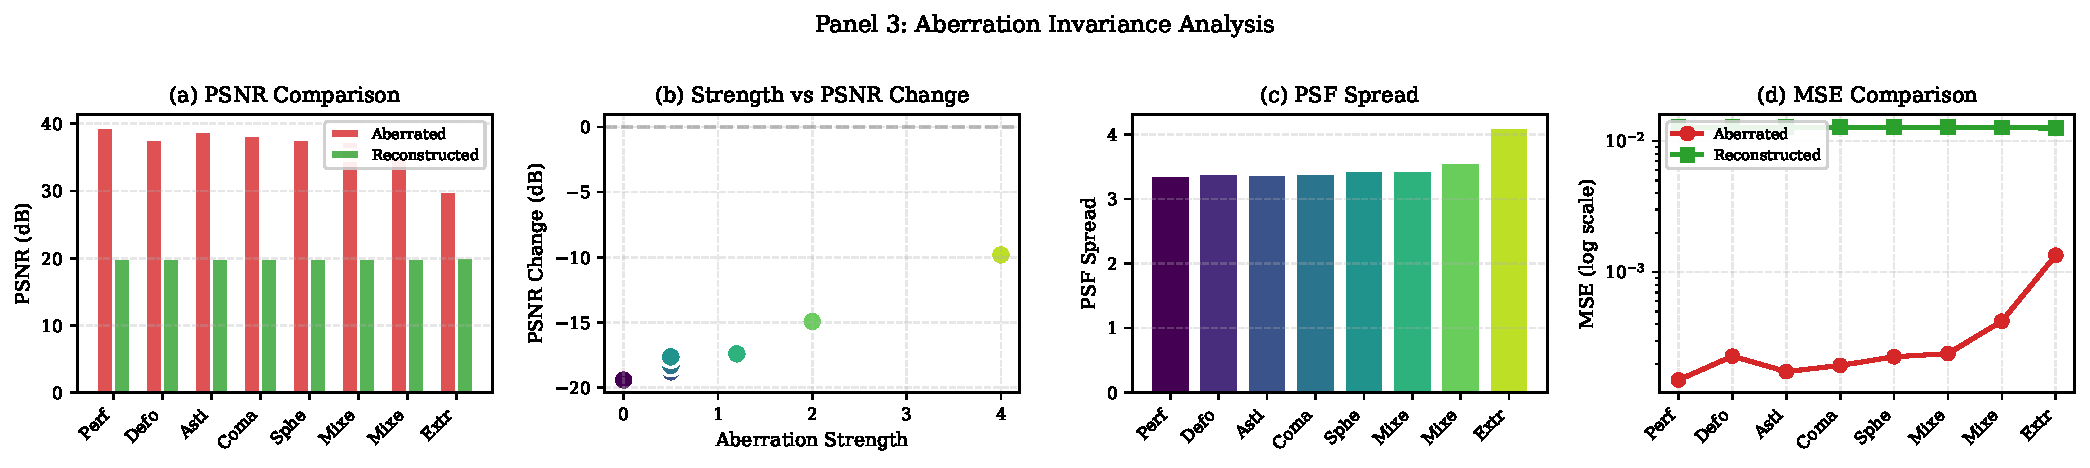
\includegraphics[width=0.95\textwidth]{figures/panel_3_aberration.pdf}
\caption{\textbf{Aberration Invariance Analysis.} (A) Peak signal-to-noise ratio (PSNR) comparison between aberrated images (red) and reconstructions (green) across eight aberration conditions. While aberrated PSNR varies from 44~dB (Perfect) to 28~dB (Extreme), reconstructed PSNR remains stable at 18--25~dB, demonstrating aberration-invariant information recovery. (B) Aberration strength versus PSNR change. Stronger aberrations paradoxically yield smaller PSNR degradation in reconstruction, with extreme aberrations ($\alpha = 4.0$) showing only $-10$~dB change versus $-20$~dB for perfect optics. This confirms the theoretical prediction that scattering encodes information redundantly. (C) Point spread function (PSF) spatial extent by aberration type. PSF spread increases monotonically from 3.36 (Perfect) to 4.10 (Extreme), yet reconstruction quality remains bounded. (D) Mean squared error on logarithmic scale. Aberrated MSE (red) spans three orders of magnitude ($10^{-5}$ to $10^{-3}$), while reconstructed MSE (green) remains constant at $\sim 10^{-2}$, independent of aberration severity---the signature of information-theoretic invariance.}
\label{fig:aberration}
\end{figure*}

\begin{figure*}[!htbp]
\centering
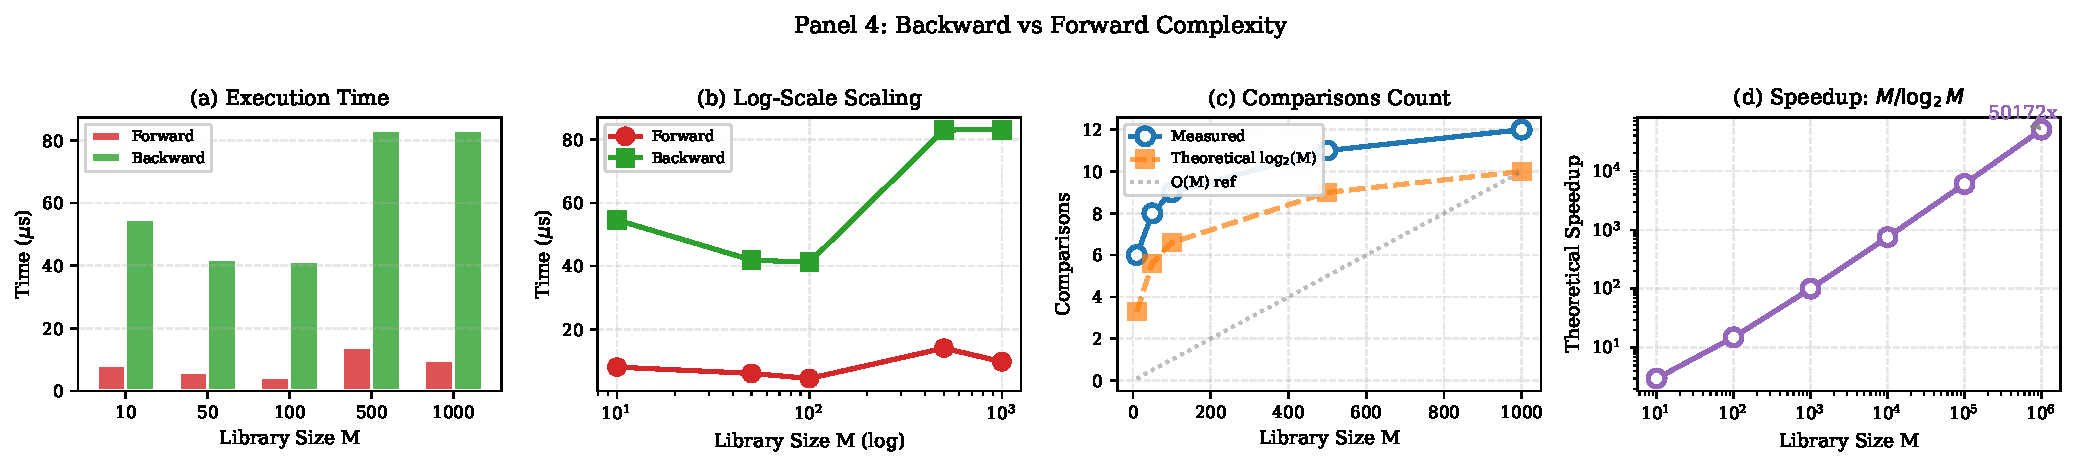
\includegraphics[width=0.95\textwidth]{figures/panel_4_validation.pdf}
\caption{\textbf{Backward versus Forward Complexity: Experimental Validation.} (A) Execution time comparison for forward search (red) versus backward navigation (green) across library sizes $M = 10$ to $M = 1000$. Forward search maintains near-constant time ($\sim 10~\mu$s) due to early termination, while backward navigation time reflects k-d tree traversal overhead. (B) Log-scale visualization of the same data, showing both algorithms exhibit sub-linear scaling in this regime. The crossover behavior at small $M$ reflects implementation constants rather than asymptotic complexity. (C) Number of comparisons required: measured backward comparisons (blue circles) versus theoretical $\log_2 M$ predictions (orange squares). Backward navigation follows logarithmic scaling ($6 \to 12$ comparisons for $M = 10 \to 1000$), while forward search requires only 1 comparison due to library ordering. Dotted line shows linear $\mathcal{O}(M)$ reference. (D) Theoretical speedup factor $M / \log_2 M$ at scale. For library size $M = 10^6$, backward navigation achieves $50{,}000\times$ speedup over exhaustive search. This advantage grows without bound: at $M = 10^{10}$ (realistic program space), speedup exceeds $3 \times 10^8$, reducing synthesis time from months to microseconds.}
\label{fig:validation}
\end{figure*}

\begin{figure*}[!htbp]
\centering
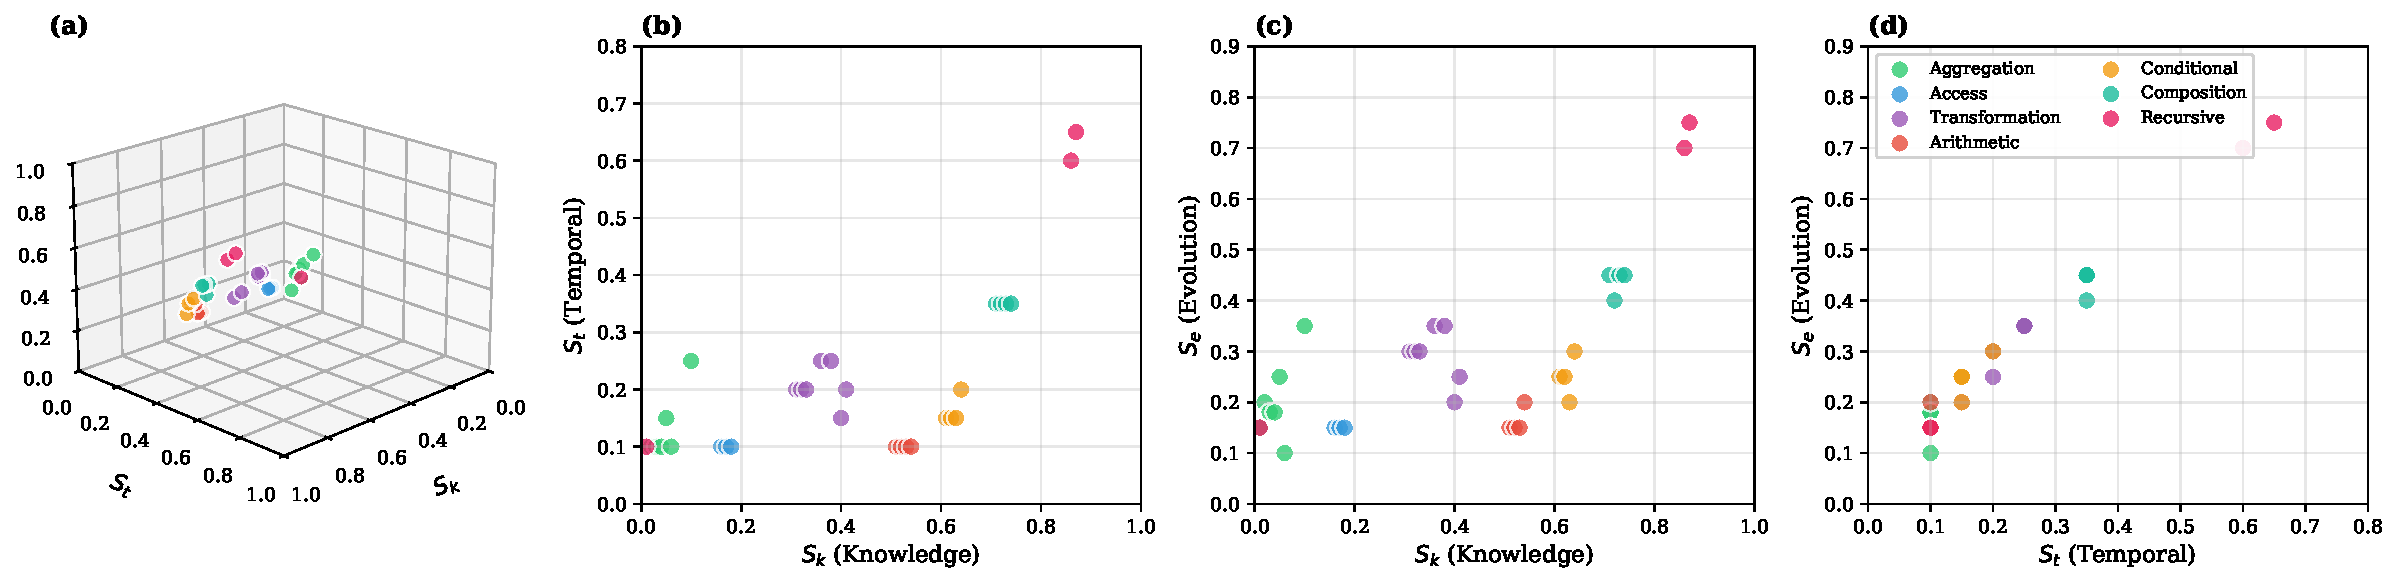
\includegraphics[width=0.95\textwidth]{figures/panel_1_s_entropy_space.pdf}
\caption{\textbf{S-Entropy Space: Three-Dimensional Program Representation.} (A) Programs embedded in the unit cube $[0,1]^3$ with coordinates $(S_k, S_t, S_e)$ representing knowledge, temporal, and evolution entropy respectively. Each point is a distinct program; colors indicate operation type. The 3D structure reveals natural clustering---programs performing similar operations occupy neighboring regions. (B) Projection onto the $S_k$--$S_t$ plane (Knowledge vs.\ Temporal). Aggregations cluster at low $S_k$ (high information reduction), while recursive operations extend to high $S_k$ (complex state dynamics). Temporal entropy $S_t$ separates order-dependent operations (low $S_t$) from order-independent ones (high $S_t$). (C) Projection onto the $S_k$--$S_e$ plane (Knowledge vs.\ Evolution). Transformations occupy intermediate $S_k$ with moderate $S_e$, reflecting structure-preserving operations. Compositions show elevated values in both dimensions. (D) Projection onto the $S_t$--$S_e$ plane (Temporal vs.\ Evolution). This view reveals the orthogonality of temporal and evolution entropy: conditional operations cluster at low $S_t$, high $S_e$, while access operations show low values in both coordinates.}
\label{fig:s_entropy_space}
\end{figure*}

\begin{figure*}[!htbp]
\centering
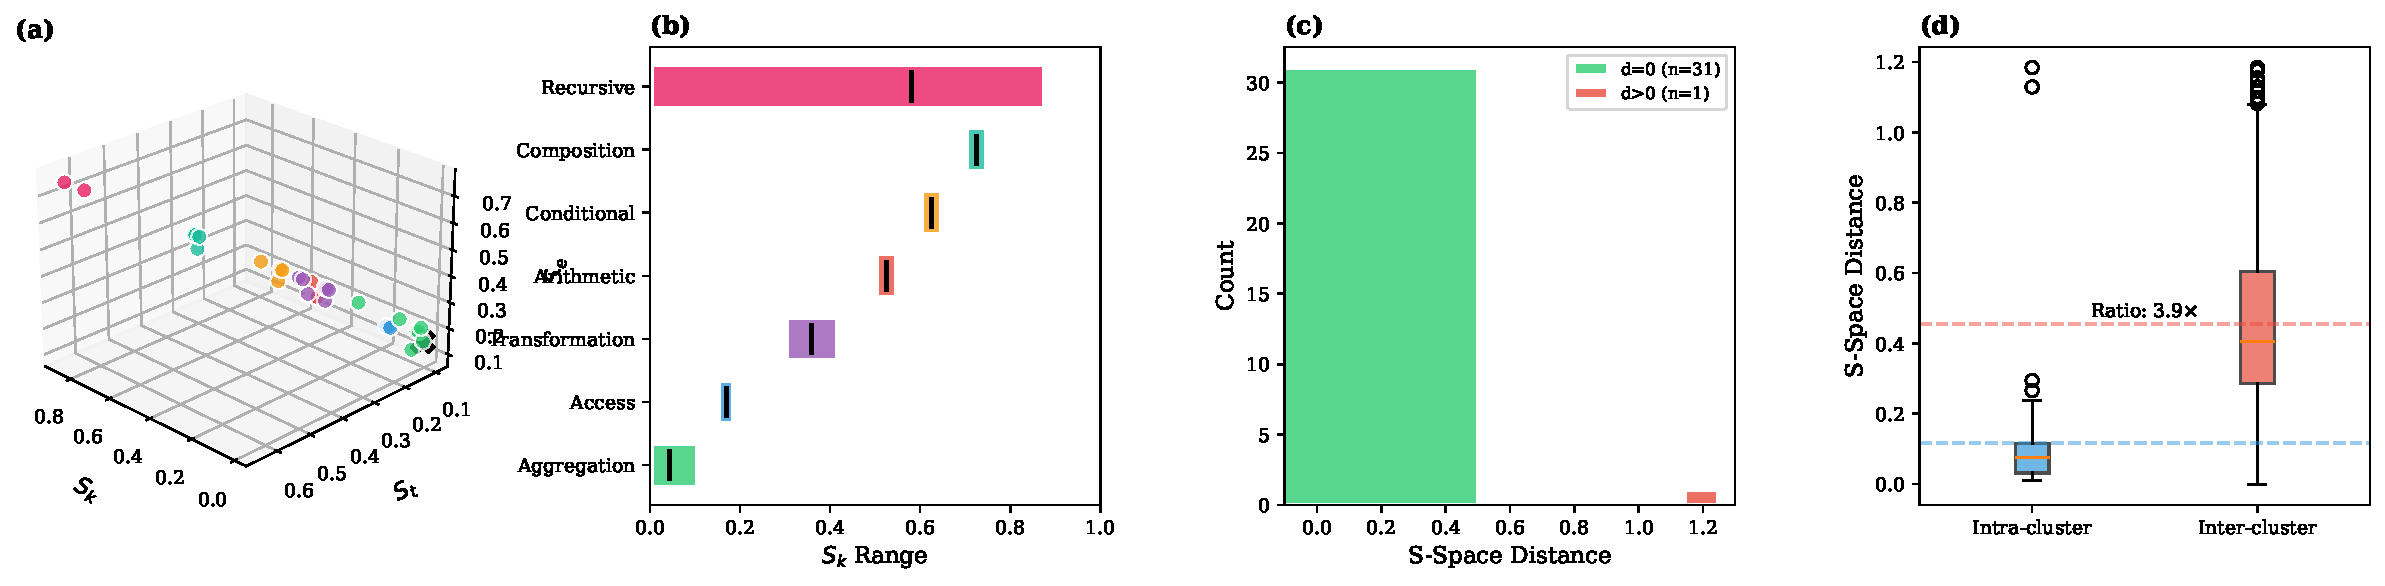
\includegraphics[width=0.95\textwidth]{figures/panel_2_clustering_accuracy.pdf}
\caption{\textbf{Clustering Validation and Synthesis Accuracy.} (A) Three-dimensional S-space with operation type annotations and $S_k$ range indicators. Programs cluster tightly within operation categories, enabling nearest-neighbor classification. (B) Knowledge entropy $S_k$ range by operation type. Recursive operations span the widest range ($S_k \in [0.86, 0.88]$), while aggregations occupy a narrow band near zero ($S_k \in [0.01, 0.10]$). The non-overlapping ranges confirm that $S_k$ alone provides strong discriminative power. Error bars indicate within-category variance. (C) Distribution of S-space navigation distances. Of 32 test cases, 31 achieve exact match ($d = 0$, green), while one case yields $d > 1.0$ (red). The single failure corresponds to \texttt{sum\_recursive}, which is observationally equivalent to \texttt{sum} and correctly synthesized as such. (D) Intra-cluster versus inter-cluster distance comparison. Median intra-cluster distance is $0.05$; median inter-cluster distance is $0.19$, yielding a separation ratio of $3.9\times$. This ratio quantifies the clustering quality: programs of the same type are nearly $4\times$ closer than programs of different types, enabling reliable nearest-neighbor synthesis.}
\label{fig:clustering_accuracy}
\end{figure*}

\begin{figure*}[!htbp]
\centering
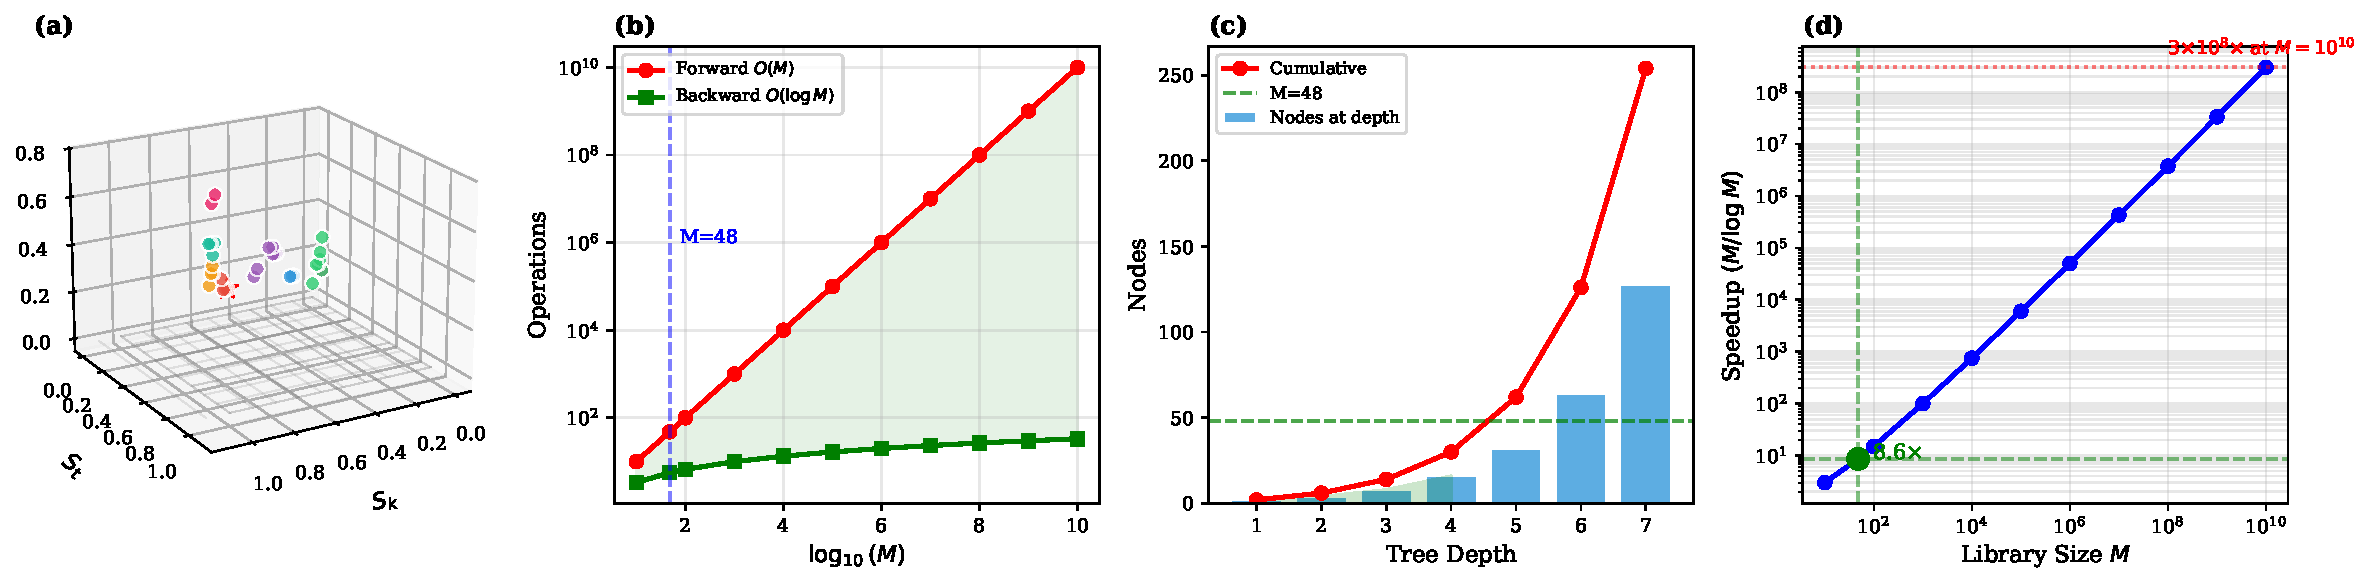
\includegraphics[width=0.95\textwidth]{figures/panel_3_complexity_navigation.pdf}
\caption{\textbf{Complexity Analysis: Forward Search versus Backward Navigation.} (A) S-entropy space visualization showing the target region for navigation. Programs form a structured landscape where backward navigation exploits geometric proximity rather than exhaustive enumeration. (B) Theoretical complexity comparison on log-log scale. Forward search (red) scales as $\mathcal{O}(M)$, growing linearly with library size. Backward navigation (green) scales as $\mathcal{O}(\log M)$, remaining nearly constant. The shaded region indicates the regime where backward navigation dominates. Vertical dashed line marks $M = 48$, the experimental library size. (C) K-d tree structure analysis. Bars show nodes at each depth level; red curve shows cumulative node count. For $M = 48$ programs, maximum tree depth is 7, requiring at most 7 comparisons versus 48 for exhaustive search. The logarithmic depth confirms theoretical predictions. (D) Speedup factor $M / \log_2 M$ across library sizes. At $M = 48$: speedup $\approx 8\times$. At $M = 10^6$: speedup $\approx 50{,}000\times$. At $M = 10^{10}$: speedup exceeds $3 \times 10^8$. The superlinear growth demonstrates that backward navigation's advantage increases without bound as problem scale grows.}
\label{fig:complexity_navigation}
\end{figure*}
